\documentclass[12pt letter]{report}
\input{./template/preamble}
\input{./template/macros}
\input{./template/letterfonts}

\title{\Huge{Memory Hierarchy and Caches}}
\author{\huge{Madiba Hudson-Quansah}}
\date{}
\usepackage{parskip}
\usepackage{tikz}
\usepackage{wheelchart}


\setcounter{tocdepth}{4}
\setcounter{secnumdepth}{4}

\begin{document}
\maketitle
\newpage
\pdfbookmark[section]{\contentsname}{too}
\tableofcontents
\pagebreak

\chapter{Memory Hierarchy}

\section{Memory Hierarchy}
The memory hierarchy is an organization of different types of memory in a computer system, based on their speed, size and cost. Starting from the top of the hierarchy, the fastest and most expensive memory is at the top, while the slowest and cheapest memory is at the bottom. The hierarchy is as follows:
\begin{description}
  \item[Registers] - Fast and small memory close to the CPU. Used to store data that is currently being processed.
  \item[Cache Memory] - Fast memory that stores frequently accessed data. It is smaller than main memory and is used to speed up access to data. Usually computers have 3 levels of cache each with increasing size and latency as you go up in levels, i.e. L1, L2 and L3 cache.
  \item[Main Memory] - Also known as RAM, it is the primary storage for data and programs that are currently in use. It is slower than cache memory but has a larger capacity.
  \item[Secondary Storage] - This is non-volatile storage that retains data even when the power is off. It is slower than main memory but has a much larger capacity. Examples include hard drives, SSDs and USB drives.
  \item[Tertiary Storage] - This is used for long-term storage of data that is not frequently accessed. It is the slowest and cheapest type of storage. Examples include magnetic tapes and optical disks.
\end{description}

\section{The Structure of Random Access Memory (RAM)}
There are two types of RAM:
\begin{description}
  \item[Static RAM (SRAM)] - Requires 6 transistors per bit of memory. It needs low power to retain state, but it is expensive and has a low density. It is used for cache memory.
  \item[Dynamic RAM (DRAM)] - Requires 1 transistor and 1 capacitor per bit of memory. It needs high power to retain state, but it is cheap and has a high density. It is used for main memory. Must be re-written after being read and must be refreshed periodically by reading and rewriting all the rows in the DRAM.
\end{description}

DRAM supports two types of access:
\begin{description}
  \item[Row Access]  - The entire row is accessed and the data is read from the row. The row is then written back to the DRAM.
  \item[Column Access] - The entire column is accessed and the data is read from the column. The column is then written back to the DRAM.
\end{description}

There are two types of DRAM:
\begin{description}
  \item[Synchronous DRAM (SDRAM)] - A clock is added to the DRAM interface to synchronize operations with the system clock. It is faster than asynchronous DRAM as with improvements in technology the system bus clock improved, increasing the rate of SDRAM operations.
  \item[Double Data Rate Synchronous DRAM (DDR)] - Is also synchronous but it performs operations on both the rising and falling edges of the clock. It is faster than SDRAM as it doubles the data rate.
\end{description}

\section{Memory Latency vs Bandwidth}

\dfn{Memory Latency}{
  The time difference between the time the request for an address is made and the time the data from that address is received. The total latency to a new row/column is the time between opening a new row of memory and accessing the column within that row. Measured in nanoseconds (ns).
}

\dfn{Memory Bandwidth}{
  The rate at which data is transferred between the memory and the CPU. Measured in millions of bytes per second (MB/s).
}

\chapter{Cache Memory}

\section{The Importance of Cache Memory}

\begin{itemize}
  \item The widening gap between CPU and memory latency is a major bottleneck in computer performance.
  \item Each instruction typically involves at least one memory access making memory access the weakest link in the instruction execution cycle.
  \item Memory bandwidth limits the instruction execution rate especially for applications that require large amounts of data to be processed.
  \item Cache memory is used to bridge the gap between CPU and memory latency by storing frequently accessed data in a small, fast memory close to the CPU.
  \item Cache memory is faster than main memory and is used to speed up access to data.
\end{itemize}

\subsection{Typical Memory Hierarchy}
\nt{}{
  \begin{description}
    \item[KiB] - 1024 bytes
    \item[MiB] - 1024 KiB
    \item[GiB] - 1024 MiB
    \item[TiB] - 1024 GiB
    \item[PiB] - 1024 TiB
  \end{description}

  \begin{description}
    \item[KB] - 1000 bytes
    \item[MB] - 1000 KB
    \item[GB] - 1000 MB
    \item[TB] - 1000 GB
    \item[PB] - 1000 TB
  \end{description}
}

\begin{figure}[htbp]
  \centering
  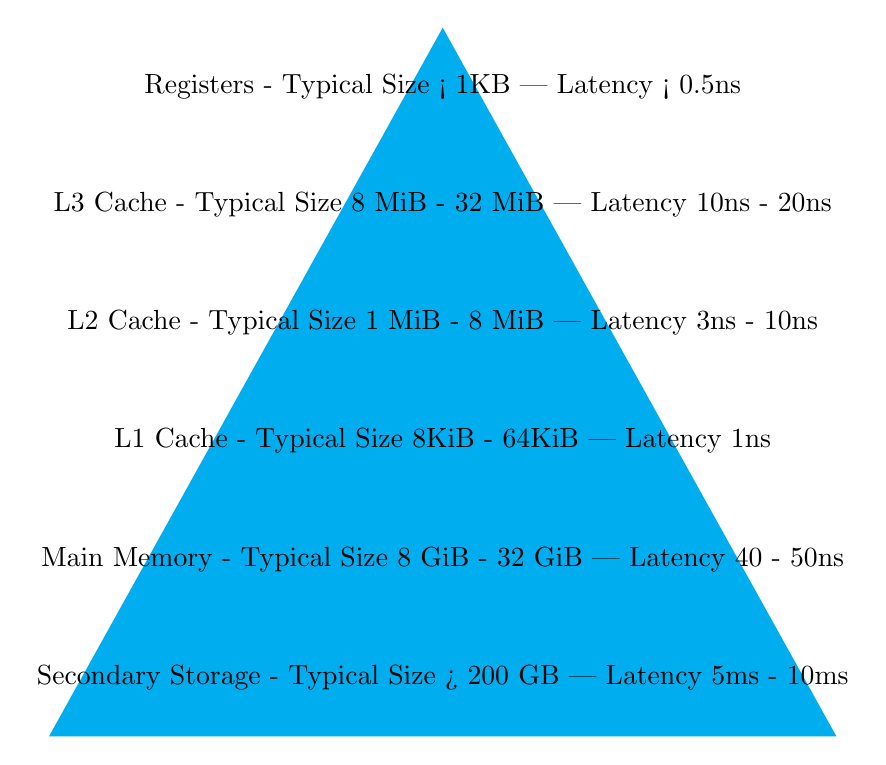
\begin{tikzpicture}
    \wheelchart[
      data=,
      slices style=\WCvarA,
      triangle proportional height={10}{9},
      value=1,
      wheel data=\WCvarB
    ]{
      cyan/Secondary Storage - Typical Size > 200 GB | Latency 5ms - 10ms,
      cyan/Main Memory - Typical Size 8 GiB - 32 GiB | Latency 40 - 50ns,
      cyan/L1 Cache - Typical Size 8KiB - 64KiB | Latency 1ns,
      cyan/L2 Cache - Typical Size 1 MiB - 8 MiB | Latency 3ns - 10ns,
      cyan/L3 Cache - Typical Size 8 MiB - 32 MiB | Latency 10ns - 20ns,
      cyan/Registers - Typical Size < 1KB | Latency < 0.5ns
    }

  \end{tikzpicture}
  \caption{Memory Hierarchy }
\end{figure}

\section{Locality of Reference}

\dfn{Locality of Reference}{
  The tendency of a program to access a relatively small portion of its address space at any given time. This means that if a program accesses a particular memory location, it is likely to access nearby memory locations in the near future.
}

\subsection{Temporal Locality (Time)}

\dfn{Temporal Locality}{
  The tendency of a program to access the same memory location multiple times within a short period of time. This means that if a program accesses a particular memory location, it is likely to access that same memory location again in the near future.
}

\subsection{Spatial Locality (\ldots and Space)}

\dfn{Spatial Locality}{
  The tendency of a program to access memory locations that are close to each other. This means that if a program accesses a particular memory location, it is likely to access nearby memory locations in the near future.
}

\section{Cache Memory}

Cache memory exploits both temporal and spatial locality by keeping frequently accessed data close to the CPU, and storing blocks consisting of multiple bytes of contiguous memory locations respectively.

Data is primary placed in a cache using block placement policies. The most common block placement policies are:
\begin{itemize}
  \item Direct Mapped Cache
  \item Set Associative Cache
  \item Fully Associative Cache
\end{itemize}
Data is then retrieved from a cache using block identification, where each block is identified via a block tag, address and an index. When a cache miss occurs data is replaced in the cache using a block replacement policy. The most common block replacement policies are:
\begin{itemize}
  \item Least Recently Used (LRU)
  \item First In First Out (FIFO)
  \item Random Replacement
\end{itemize}

\subsection{Block Placement Policies}

\dfn{Cache Block / Cache Line}{
  Unit of data transfer between main memory and a cache. The larger the block size the less tag overhead and the more data that can be transferred at once. However, larger block sizes can lead to more cache misses as the data may not be used immediately. Typically 64 bytes in size
}

\dfn{Block}{
  Unit of data transfer between a cache and memory.
}

\subsubsection{Direct Mapped Cache}

\dfn{Direct Mapped Cache}{
  Each block can only be placed in exactly one location in the cache. Using this policy memory addresses are divided into block addresses and block offsets, identifying the block in memory and the offset to access specific bytes within that block respectively. A block address is then further subdivided into an index and a tag used for direct cache access and the most significant bits of the address respectively, i.e. the index is calculated as
  \[
    \text{Index} = \text{Block Address} \mod \text{Number of Cache Lines}
  \]
}

\dfn{Cache Hit}{
  A cache hit occurs when the block is found in the cache. The index is used to access the cache block and address tag is compared against the stored tag in the cache. If the tags match, the data is returned from the cache. If the tags do not match, a cache miss occurs and the data is fetched from main memory.
}

If the number of cache blocks is $2^{n}$ then $n$ bits are used for the cache index, if the number of bytes in a block is $2^{b}$ then $b$ bits are used for the offset, and depending on the size of the address the remaining bits are used for the tag, i.e. if 32 bit addresses then $\text{Tag} = 32 - n - b$. Generally:
\[
  \text{Tag bits} = \text{Address bits} - \text{Index bits} - \text{Offset bits}
\]
The cache data size is therefore $2^{n + b}$ bytes

For example if a direct mapped cache has 256 blocks, and each block is 16 bytes, assuming 32 bit addresses:
\begin{align*}
  \text{Index}  & = 2^{n} =256 \\
                & = n = 8      \\
  \text{Offset} & = 2^{b} = 16 \\
                & = n = 4      \\
  \text{Tag}    & = 32 - 8 - 4 \\
                & = 20         \\
\end{align*}
Therefore the division is:
\begin{table}[htbp]
  \begin{center}
    \begin{tabular}{|c|c|c|}
      \hline
      \texttt{Tag} & \texttt{Index} & \texttt{Offset} \\
      \hline
      20 bits      & 8 bits         & 4 bits          \\
      \hline
    \end{tabular}
  \end{center}
\end{table}
Then computing the tag, index and offset for the address $0x01FFF8AC$ we get:
\begin{align*}
  \text{Tag}    & = 0x01FFF \\
  \text{Index}  & = 0x8A    \\
  \text{Offset} & = 0xC     \\
\end{align*}

\section{Write Policies}

\dfn{Write Through}{
  Data is written to both the cache and main memory at the same time. This ensures that the data in main memory is always up to date, but it can slow down the system as both writes must be completed before the CPU can continue processing. Memory always has the latest data which simplifies data coherency. Only a valid bit is required to indicate if the data is valid in the cache.
}

\dfn{Write Back}{
  Data is written to the cache only and is marked as dirty. The data is then written to main memory only when the block is replaced in the cache. This can speed up the system as only one write is required, but it can lead to data inconsistencies if the data in main memory is not updated. Memory may not have the latest data which complicates data coherency. Uses less memory bandwidth as only one write is required. Both valid and modified bits are required to indicate if the data is valid and modified in the cache respectively.
}

\dfn{Modified Bit}{
  A bit used to indicate if the data in the cache has been modified. If the modified bit is set, the data in the cache is different from the data in main memory and must be written back to main memory before the block is replaced.
}

\section{Replacement Policies}

Direct Mapped caches have no selection alternatives for replacement as each block can only be placed in one location in the cache. However, set associative and fully associative caches have multiple locations for each block and therefore have to select which block to replace when a cache miss occurs. The most common replacement policies are:

\dfn{Random Replacement}{
  Candidate blocks are randomly selected for replacement. One counter for all sets (0 to $m-1$), where $m$ is the number of sets. The counter is incremented for each access and the block with the same index as the counter is replaced. This policy is simple to implement but can lead to poor performance as it does not take into account the usage patterns of the blocks. On a cache miss the block replaced is specified by the counter.
}

\dfn{First In First Out (FIFO)}{
  The oldest block in the cache is replaced. This policy is simple to implement but can lead to poor performance as it does not take into account the usage patterns of the blocks. On a cache miss the block replaced is specified by the index of the block in the cache.
}

\dfn{Least Recently Used (LRU)}{
  The block that has been unused for the longest time is replaced. This policy is more complex to implement as it requires keeping track of the usage patterns of the blocks. On a cache miss the block replaced is specified by the index of the block in the cache. The LRU policy can be implemented using a stack or a counter for each block. With $m$ blocks per set there are $m!$ possible permutations of the blocks. Pure LRU is to costly to implement when $m > 2$, therefore an approximate method is used.
}


\end{document}
